\chapter{Results } \label{Results}

\begin{itemize}
  \item After doing successful set-up and receiver-calibration procedures, 20*100 readings of length 12280 points of drone and non-drone signals respectively were successfully captured and stored into the file system for training of the model.
    \item some captured sample drone and non-drone signals are plotted below.
    \begin{figure}[H]
      \label{drone}
      \begin{subfigure}{0.5\textwidth}
        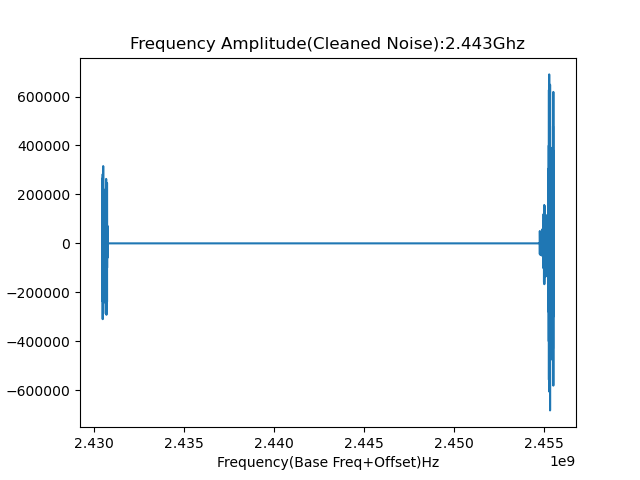
\includegraphics[width=0.9\linewidth ]{images/drone_2.413Ghz-FA-4.00.png}
        \label{fig:subim1.1}
      \end{subfigure}
      \begin{subfigure}{0.5\textwidth}
        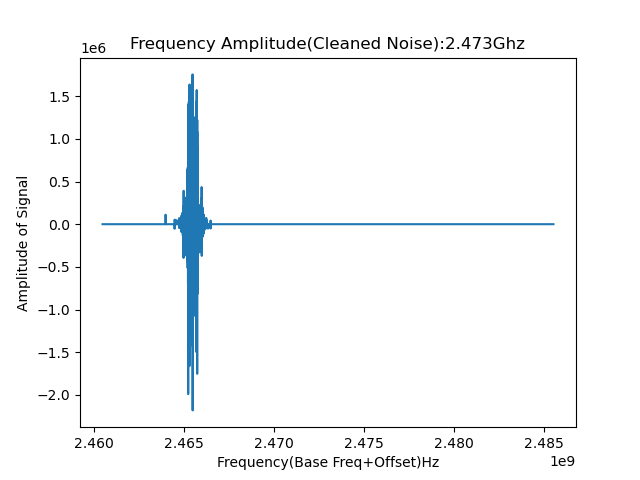
\includegraphics[width=0.9\linewidth]{images/drone_2.413Ghz-FA-8.00.png}
        \label{fig:subim2.1}
      \end{subfigure}

      \begin{subfigure}{0.5\textwidth}
        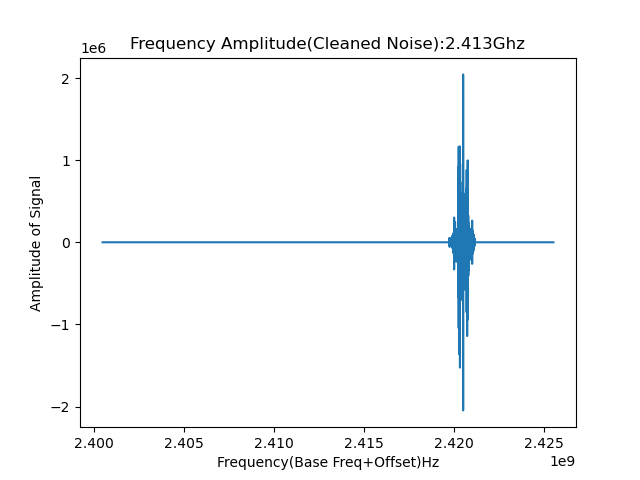
\includegraphics[width=0.9\linewidth]{ images/drone_2.413Ghz-FA-10.00.png }
        \label{fig:subim3.1}
      \end{subfigure}
      \begin{subfigure}{0.5\textwidth}
        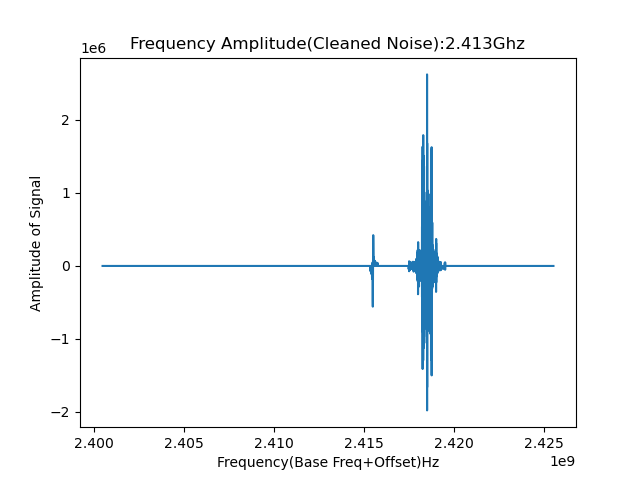
\includegraphics[width=0.9\linewidth]{ images/drone_2.413Ghz-FA-16.00.png }
        \label{fig:subim4.1}
      \end{subfigure}

        \centering
      \begin{subfigure}{0.5\textwidth}
        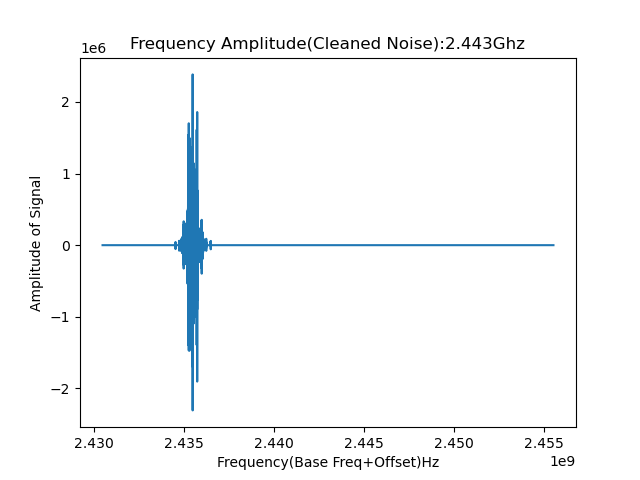
\includegraphics[width=0.9\linewidth]{ images/drone_2.443Ghz-FA-0.00.png }
        \label{fig:subim5.1}
      \end{subfigure}
      \caption{Sample drone signals}
      \label{fig:image2.1}
    \end{figure}

    \begin{figure}[H]
      \label{drone}
      \begin{subfigure}{0.5\textwidth}
        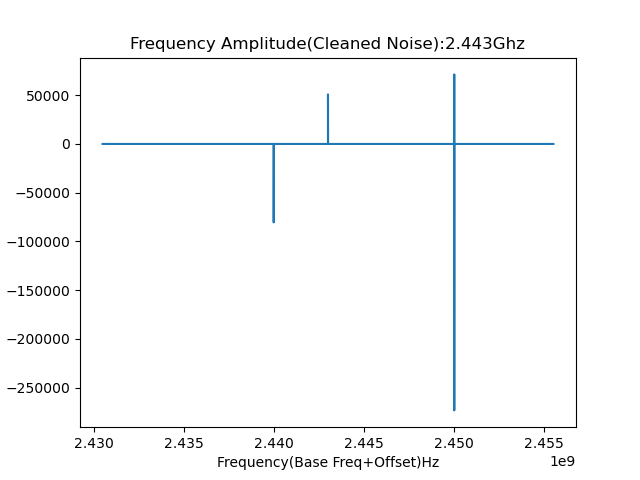
\includegraphics[width=0.9\linewidth ]{ images/nondrone_2.413Ghz-FA-5.00.png }
        \label{fig:subim1}
      \end{subfigure}
      \begin{subfigure}{0.5\textwidth}
        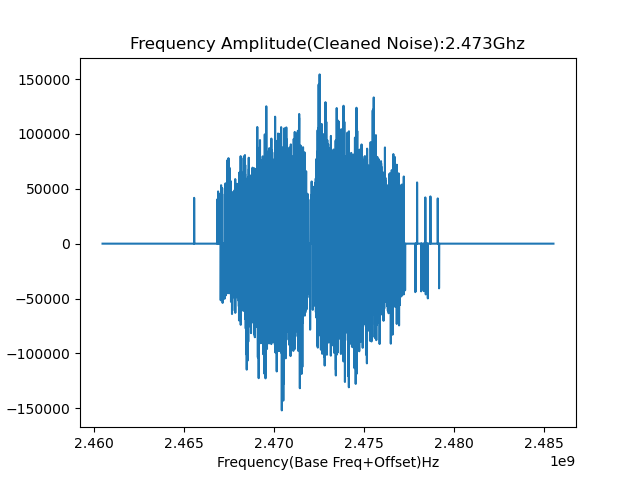
\includegraphics[width=0.9\linewidth]{ images/nondrone_2.413Ghz-FA-6.00.png }
        \label{fig:subim2}
      \end{subfigure}

      \begin{subfigure}{0.5\textwidth}
        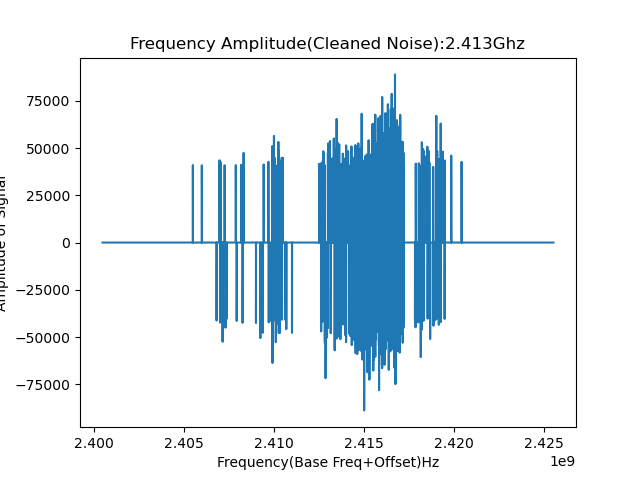
\includegraphics[width=0.9\linewidth]{ images/nondrone_2.413Ghz-FA-19.00.png }
        \label{fig:subim3}
      \end{subfigure}
      \begin{subfigure}{0.5\textwidth}
        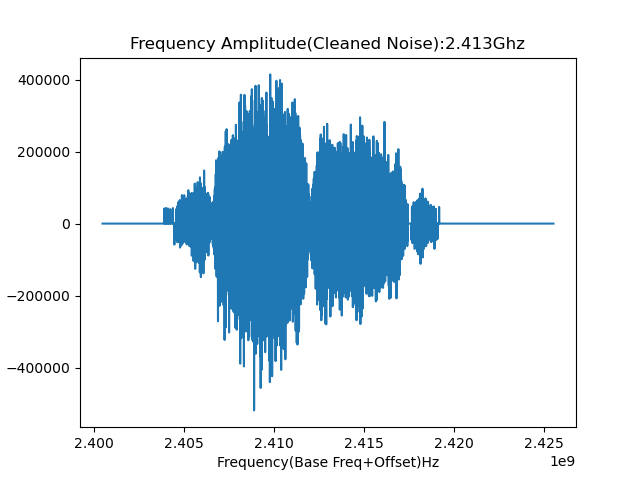
\includegraphics[width=0.9\linewidth]{ images/nondrone_2.443Ghz-FA-19.00.png }
        \label{fig:subim4}
      \end{subfigure}

        \centering
      \begin{subfigure}{0.5\textwidth}
        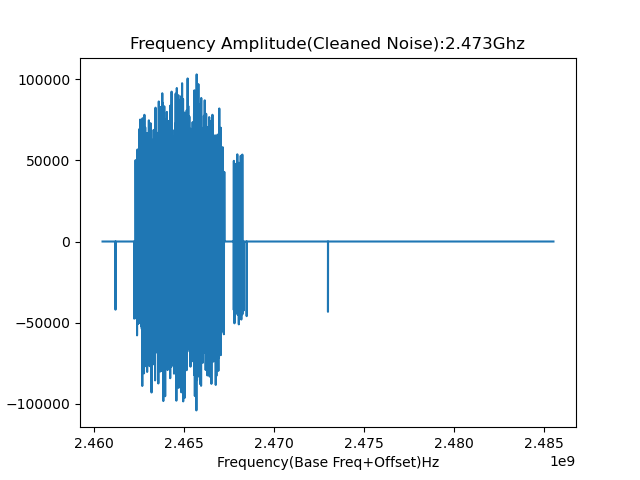
\includegraphics[width=0.9\linewidth]{ images/nondrone_2.473Ghz-FA-12.00.png }
        \label{fig:subim5}
      \end{subfigure}
      \caption{Sample Non-Drone signals}
      \label{fig:image2}
    \end{figure}
  \item As seen above, drone and non-drone signals have a distinct frequency signature in the same frequency bands with occasional frequency overlaps.

\item This is used as one of the primary criteria during classification, which is distinct from their energy signal levels.
\end{itemize}
\begin{itemize}
  \item After successful creation and dataset manipulation, the model is trained for a batch size of 1665 readings per epoch. After a successful run of 15 epochs, the model prediction accuracy and loss function are shown as graphically plots as follows:
    \begin{figure}[H]
      \begin{subfigure}{0.5\textwidth}
        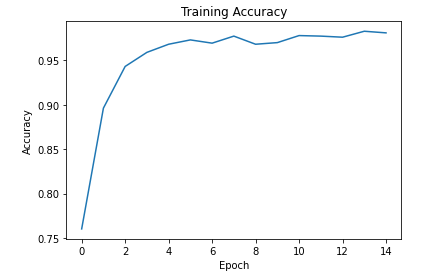
\includegraphics[width=0.9\linewidth]{ images/Model-Accuracy.png }
        \caption{Model Accuracy}
        \label{fig:subim5}
      \end{subfigure}
      \begin{subfigure}{0.5\textwidth}
        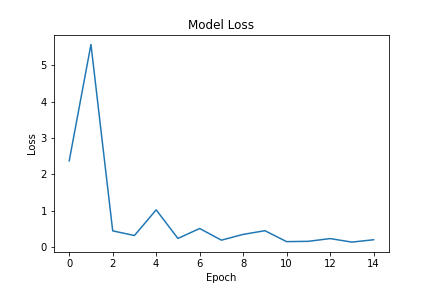
\includegraphics[width=0.9\linewidth]{ images/Model-Loss-Acc.png }
        \caption{Model Loss}
        \label{fig:subim5}
      \end{subfigure}
    \end{figure}

  \item As seen above, the model tends to nearly maintain a relatively low loss while maintaining relatively high accuracy values over the range of the epoch cycles.

  \item Due to frequent data shuffling and randomization, there are some sudden changes in loss and accuracy values which signify that the model is prevented from overtraining and memorizing the correct labels over the epoch cycles while training.
\end{itemize}

\begin{itemize}
\item After successful data and model loading, the model can predict successfully under which category the inputs came.

\item The model can give output class values in integer form that are later mapped to an array containing the category names as its index.

eg: '0' corresponds to non-drone and '1' corresponds to FlySky drone.

\item The jammer section later uses this classification to target the corresponding spectrum in which the drone is operating.
\end{itemize}

